\renewcommand{\theequation}{\theenumi}
\renewcommand{\thefigure}{\theenumi}
\renewcommand{\thetable}{\theenumi}
\begin{enumerate}[label=\thesection.\arabic*.,ref=\thesection.\theenumi]
\numberwithin{equation}{enumi}
\numberwithin{figure}{enumi}
\numberwithin{table}{enumi}


\item Consider a Binary Symmetric Channel (BSC) with probability of error being p.To transit a bit, say 1,we transmit a sequence of three 1s.The receiver will interpret the received sequence to represent 1 if at least if at least two bits are 1.The probability that the transmitted bit will be received in error is
\begin{enumerate}
\item $p^3 + 3 p^2\brak{1-p}$ 

\item $p^3$

\item $\brak{1-p}^3$

\item $p^3+p^2\brak{1-p}$
\end{enumerate}

%
\solution
Given that, the CDF of the given random variable is
$$
F_X(x)=\begin{cases}
			x/2, & 0<x<\frac{1}{2}\\
            x, & \frac{1}{2}\leq x\leq 1
		 \end{cases}
$$
% \begin{figure}[h]
%     \includegraphics[width = 8cm]{images/Assignment_2.png}
% \end{figure}
that means probability of the random variable being $m$ is
\begin{align}
\Pr(X = m) =F_X(m) -  \lim_{t \to m^-}F_X(t)
\end{align}
Hence the probability value at $ X =\frac{1}{2}$ is
\begin{align}
    \Pr(X = 1/2) &= F_X\brak{\dfrac{1}{2}} -\lim_{t \to \frac{1}{2}^-}F_X(t)\\
    &= \frac{1}{2} - \lim_{x \to \frac{1}{2}^-} \frac{x}{2}\\
    &= \frac{1}{2} - \frac{1}{4}\\
    &= \frac{1}{4} = 0.25
\end{align}




\item The input X to the binary Symmetric Channel (BSC) shown in Fig. \ref{fig:7} is '1' with probability 0.8. The cross-over probability is $\dfrac{1}{7}$. If the received bit Y=0, the conditional probability that '1' was transmitted is........\\


\begin{figure}[!h]
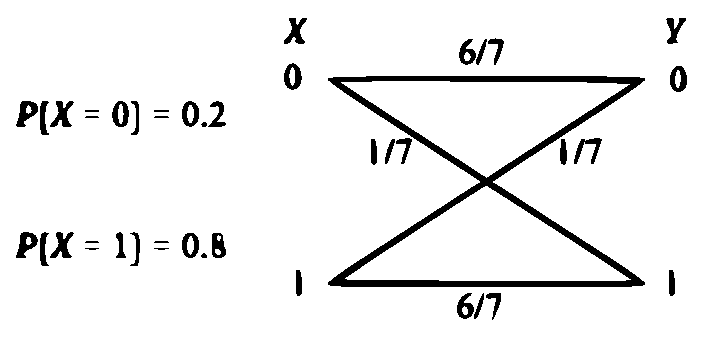
\includegraphics[width=\columnwidth]{./figs/figure7.eps}
\caption{}
\label{fig:7}
\end{figure}
%
\solution
\begin{align}
    \pr{X = 1|Y = 0}&=\frac{\pr{\{X=1\}\{Y=0\}}}{\pr{Y=0}} \label{eq:1}\\
    \pr{Y = 0|X = 1}&=\frac{\pr{\{X=1\}\{Y=0\}}}{\pr{X=1}} \label{eq:2}
\end{align}
From \eqref{eq:2},
\begin{align}
    \pr{\{X=1\}\{Y=0\}} &= \pr{Y = 0|X = 1}\pr{X=1} \label{eq:3}
\end{align}
Substituting \eqref{eq:3} in \eqref{eq:1},
\begin{align}
    \pr{X = 1|Y = 0} &= \frac{\pr{Y = 0|X = 1}\pr{X=1}}{\pr{Y=0}} \label{eq:7}
\end{align}
Given data,
\begin{align}
    \pr{Y = 0|X = 1} =\frac{1}{7}, \pr{Y =0|X=0}=\frac{6}{7} \label{eq:4}
\end{align}
\begin{multline}
    \pr{Y=0} = \pr{Y = 0|X = 1}\pr{X=1} +\\ \pr{Y = 0|X = 0}\pr{X=0} \label{eq:6}
\end{multline}
Substituting the values from \eqref{eq:4} and the data given in the question in \eqref{eq:6},
\begin{align}
    \pr{Y=0} &= \frac{2}{7} \label{eq:5}
\end{align}
Substituting \eqref{eq:4}, \eqref{eq:5} and the data given in the question in \eqref{eq:7},
\begin{align}
    \pr{X = 1|Y = 0} = 0.4
\end{align}


%
\item A binary symmetric channel (BSC) has a transition probability of $\dfrac{1}{8}$. If the binary transmit symbol X is such that $P(X=0)=\dfrac{9}{10}$, then the probability of error for an optimum receiver will be
\begin{enumerate}
\begin{multicols}{4}
\setlength\itemsep{2em}
\item $
\dfrac{7}{80}
$
\item $
\dfrac{63}{80}
$
\item $
\dfrac{9}{10}
$
\item $
\dfrac{1}{10}
$
\end{multicols}
\end{enumerate}
\solution
\input{solutions/24/latex2.tex}
%
\item A digital communication system uses a repetition code for channel encoding/decoding. During transmission, each bit is repeated three times(0 is transmitted as 000, and 1 is transmitted as 111). It is assumed that the source puts out symbols independently and with equal probability. The decoder operates as follows: In a block of three received bits, if the number of zeros exceeds the number of ones, the decoder decides in favour of a 0, and if the number of ones exceeds the number of zeros, the decoder decides in favour of a 1. Assuming a binary symmetric channel with crossover probability p = 0.1, the average probability of error is ........
%
\\
\solution
Let Y be the bit sent by the sender and X be the number of 1's received by the receiver and p = 0.1 is the crossover probability
\\
{Case 1: Y = 0}
\begin{align}
    \Pr(X = i) &= \binom{n}{i}\times p^i\times (1-p)^{n-i}
\end{align}
When $X \geq 2 $ the receiver interprets it as 1, which is an error. And by Total Probability theorem we have\\
\begin{align}
P_1 = \frac{P(X = 2) + P(X = 3)}{\sum_{i=0}^3P(X = i)}
\end{align}
where $P_1$ is the probability of error when Y = 0
\\
{Case 2: Y = 1}
\begin{align}
\Pr(X = i) &= \binom{n}{i}\times p^{n-i}\times (1-p)^i
\end{align}
When $X \leq 1 $ the receiver interprets it as 0, which is an error. And by Total Probability theorem we have
\begin{align}
P_2 = \frac{\Pr(X = 0) + \Pr(X = 1)}{\sum_{i=0}^3\Pr(X = i)}
\end{align}
where $P_2$ is the probability of error when Y = 1
\begin{multline}
\sum_{i=0}^3\Pr(X = i) = 1\times 0.9^3 + 3\times 0.1\times 0.9^2 \\
+ 3\times 0.1^2 \times 0.9 + 1\times 0.1^3 = 1
\end{multline}
\begin{align}
P_1 &= 0.028\\
P_2 &= 0.028
\end{align}
The average probability is 
\begin{multline}
P_{avg} = \Pr(Y = 0)\times P_1 +\Pr(Y = 1)\times P_2\\ = 0.028 \end{multline}
\begin{table}[!ht]
\centering
\resizebox{\columnwidth}{!}{
\begin{tabular}{|c|c|c|c|c|c|}
\hline
     &X&0&1&2&3  \\
     \hline
     Y=0&$\Pr(X)$&0.729&0.243&0.027&0.001\\
     \hline
     Y=1&$\Pr(X)$&0.001&0.027&0.243&0.729\\
     \hline
\end{tabular}}
\caption{Probability of number of 1's recieved  }
\label{ec40:table:1}
\end{table}
%
\item Consider the Z-channel given in Fig. \ref{fig:1}. The input is 0 or 1 with equal probability.
\begin{figure}[!h]
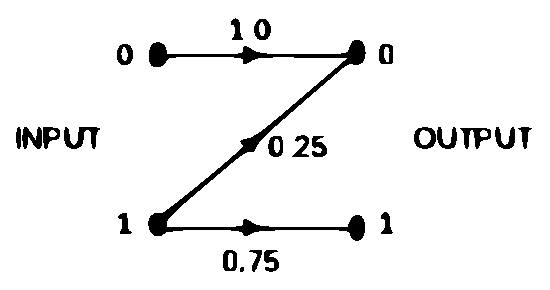
\includegraphics[width=\columnwidth]{./figs/figure1.eps}
\caption{}
\label{fig:1}
\end{figure}
If the output is 0, the probability that the input is also 0 equals......

\item A sender(S) transmits a signal,which can be one of two kinds: H and L with probabilities 0.1 and 0.9 respectively, to a receiver (R).\\
In the graph below,the weight of an edge(u,v) is the probability of receiving v when u is transmitted,where u,v $\in$ \{H,L\}.For example the probability that the received signal is L given the transmitted signal is H is 0.7.
\begin{figure}[h!]
    \centering
    \includegraphics[width=\columnwidth]{solutions/cs/2021/figures/qnfigure.png}
\end{figure}
%
If the received signal is H, the probability that the transmitted signal was H is \underline{\quad\quad\quad} ?

\solution
Given X and Y be two continuous random variables with the joint probability density function
\begin{align}
    f\left(x,y\right)=\begin{cases}
    2 \quad  0<x+y<1 ,x>0 ,y>0\\
    0 \quad  \textrm{elsewhere}\\
    \end{cases}
\end{align}
% \begin{figure}[h]
%     \centering
%     \includegraphics[scale=0.2]{f(x,y)_graph.png}
%     \caption{$f\left(x,y\right)$}
%     \label{ec/75/fig:f(x,y)}
% \end{figure}

we know that
\begin{align}
    P\left(\left(x,y\right)\in A\right)=\int \int _{A}f\left(x,y\right) dx dy \quad  A \in \mathbb{R}^2
\end{align}
from given information\\
for positive $x$ and $y$
\begin{align}
    0<x+y<\dfrac{1}{2}  \Rightarrow 0<x<\dfrac{1}{2}-y
\end{align}
so using eq(0.0.3)
\begin{align}
    P\left(x+y < \dfrac{1}{2}\right)=\int_{0}^{\frac{1}{2}} \int _{0}^{\frac{1}{2}-y}f(x,y) dx dy\\
    =\int_{0}^{\frac{1}{2}} \int _{0}^{\frac{1}{2}-y} 2 \quad dx dy
    =\int_{0}^{\frac{1}{2}} \left(  2 x \quad \big|_{0}^{\frac{1}{2}-y} \right)  dy\\
    =\int_{0}^{\frac{1}{2}}   2 \left(\frac{1}{2}-y\right) \quad    dy
    =2\left( \frac{1}{2} y - \frac{y^2}{2}  \right) \big|_{0}^{\frac{1}{2}}\\
    = \left( \frac{1}{2} - \frac{1}{4}\right) = \frac{1}{4} 
\end{align}
Therefore 
\begin{align}
    P\left(X+Y<\dfrac{1}{2}\right)=\dfrac{1}{4}
\end{align}
\begin{align}
\intertext{volume under the graph which contains the region} X+Y<\dfrac{1}{2} \quad \text{gives us} \quad P\left(X+Y<\dfrac{1}{2}\right) \\
 P\left(X+Y<\dfrac{1}{2}\right)= \text{Area of the base . height}
 \end{align}
 
Area of the base triangle is 
\begin{align}
 \dfrac{1}{2}.\textit{height}.\textit{base} =\dfrac{1}{2}.\dfrac{1}{2}.\dfrac{1}{2}
 \end{align}
 \begin{align}
\text{volume = Area . height}=\dfrac{1}{8}. 2= \dfrac{1}{4}
\end{align}
%The volume under the graph which contains the region $X+Y<\dfrac{1}{2}$ %gives us $P\left(x+y<\dfrac{1}{2}\right)$\\
%$P\left(x+y<\dfrac{1}{2}\right)=$ Area of the base . height\\
%Area of the base triangle is $\dfrac{1}{2}.\textit{height}.\textit{base}$%$= \dfrac{1}{2}.\dfrac{1}{2}.\dfrac{1}{2}$\\
%volume = Area . height $= \dfrac{1}{8}. 2= \dfrac{1}{4}$

\begin{figure}[h]
    \centering
    %\columnwidth
    \includegraphics[width=\columnwidth]{solutions/ec/75/P(x+y_2)_graph.png}
    \caption{$P\left(x+y<\dfrac{1}{2}\right)$}
    \label{ec/75/fig:p(x+y<1/2)}
\end{figure}





%
\item A binary symmetric channel $\brak{BSC}$ has a transition probability of $\frac{1}{8}$. If the binary symbol X is such that P $\brak{X = 0}$ = $\frac{9}{10}$ , then the probability of error for an optimum receiver will be 
\begin{enumerate}[]
\begin{multicols}{2}
\setlength\itemsep{0.1em}
\item $\frac{7}{80}$ \label{ec2012-35option A}
\item $\frac{63}{80}$ \label{ec2012-35option B}
\item $\frac{63}{80}$ \label{ec2012-35option C}
\item  $\frac{1}{10}$ \label{ec2012-35option D}
\end{multicols}
\end{enumerate}
%
\solution
Probability of  transition,p is given by
\begin{align}
    p =  \frac{1}{8} \\
    \pr{X = 0} = \frac{9}{10} \\
    \pr{X = 1} = \frac{1}{10}
\end{align}
\begin{center}
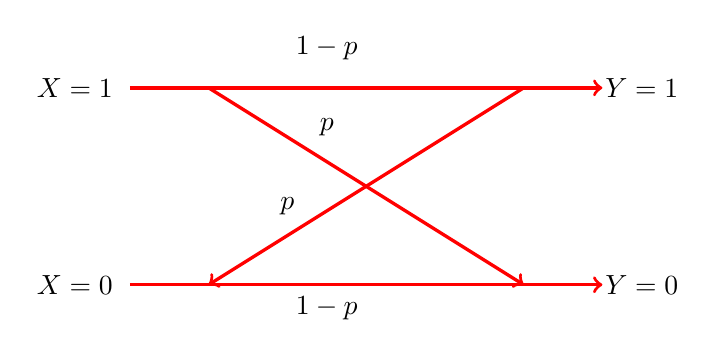
\begin{tikzpicture}
\begin{scope}[red,very thick,->]
    \draw  (0,0) -- (6,0);
   \draw (1,0) -- (5,-2.5);
   \draw (5,0) -- (1,-2.5);
   \draw (0,-2.5) -- (6,-2.5);
\end{scope}
   \node at (-0.7,0) {$\displaystyle X = 1 $};
   \node at (6.5,0)  {$\displaystyle Y = 1$};
   \node at (-0.7,-2.5) {$\displaystyle X = 0$};
   \node at (6.5,-2.5) {$\displaystyle Y = 0$};
   \node at (2.5,0.5) {$\displaystyle 1-p$};
   \node at (2.5,-2.8) {$\displaystyle 1-p$};
   \node at (2.5,-0.5) {$\displaystyle p$};
   \node at (2,-1.5) {$\displaystyle p$};
\end{tikzpicture}
\end{center}
\begin{center}
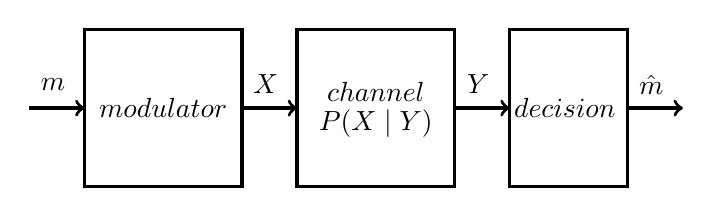
\begin{tikzpicture}
\begin{scope}[black,very thick,->]
         \draw (-0.3,0) rectangle (1.7,2); 
    \draw (2.4,0) rectangle  (4.4,2);
    \draw [->] (1.7,1) -- (2.4,1);
    \draw [->] (4.4,1) -- (5.1,1);
    \draw (5.1,0) rectangle (6.6,2);
    \draw [->] (6.6,1) -- (7.3,1);
    \draw [->] (-1,1) -- (-0.3,1);
\end{scope}
    \node at (1.5,1.5) {$\displaystyle $};
    \node at (1.5,0.5) {$\displaystyle $};
    \node at  (0.7,1)  {$\displaystyle modulator$};
    \node at  (-0.7,1.3)  {$\displaystyle m$};
    \node at  (2,1.3)  {$\displaystyle X$};
    \node at  (4.7,1.3)  {$\displaystyle Y$};
    \node at  (6.9,1.3)  {$\displaystyle \hat{m}$};
    \node at  (5.8,1)  {$\displaystyle decision$};
    \node at  (3.4,1.2)  {$\displaystyle channel$};
    \node at  (3.4,0.8)  {$\displaystyle P(X \mid Y)$};
\end{tikzpicture}
(here $m$ and $X$ can be considered similar)
\end{center}
$\therefore$ Probability of error is defined as 
\begin{align}
    P_e = \pr{\hat{m} \neq m}
\end{align}
Probability of being correct is defined as
\begin{align}
    P_c & = 1 - P_e  \\
        & = 1 - \pr{\hat{m} \neq m} \\
        & = \pr{\hat{m} = m} 
\end{align}
Optimum detector maxmize $P_c$ or equivalently minimize $P_e$ \\ Probability of making correct decision, for a given received y 
\begin{align}
    P_c & = \pr{\hat{m} = m} \\
        & = p(m_i \mid y) p(y) \\
        & = p(x_i \mid y) p(y)
\end{align}
Using Bayes theorem,
\begin{align}
    P_c & = p(y \mid x_i) p(x_i)
\end{align}
To maximize $P_c$ we use \textbf{Maximum a Posterior Detector (MAP)} rule , for a given $Y$
\begin{align}
    \hat{m} \implies m_i \ \ if \ \ \frac{p(y \mid x_i) p(x_i)}{p(y \mid x_j) p(x_j)} \geq 1
\end{align}
Now , when Y = 1 then $\hat{m}$ = 0 if
 
\begin{align}
    \frac{p(y = 1 \mid x = 0) p(x=0)}{p(y =1  \mid x = 1) p(x=1)} \geq 1 \\
\implies  \frac{p(y = 1 \mid x = 0) p(x=0)}{p(y =1  \mid x = 1) p(x=1)} \\
= \frac{\frac{1}{8} \cdot \frac{9}{10}}{\frac{7}{8} \cdot \frac{1}{10}}  \\
= \frac{9}{7} \geq 1
\end{align}
when Y = 0 then $\hat{m}$ = 0 if
\begin{align}
        \frac{p(y = 0 \mid x = 0) p(x=0)}{p(y = 0  \mid x = 1) p(x=1)} \geq 1 \\
\implies  \frac{p(y = 0 \mid x = 0) p(x=0)}{p(y = 0 \mid x = 1) p(x=1)} \\
= \frac{\frac{7}{8} \cdot \frac{9}{10}}{\frac{1}{8} \cdot \frac{1}{10}}  \\
= 63 \geq 1        
\end{align}
In both cases MAP detector suggest that message will be $\hat{m}$ = 0 \\
$\therefore$ probability of error 
\begin{multline}
    P_e  = \pr{\hat{m} \neq 0 \mid X = 0 } \pr{X = 0} \\ + \pr{\hat{m} \neq 1 \mid X = 1} \pr{X = 1} 
\end{multline}
\begin{align}    
    & = 0 + 1 \cdot \frac{1}{10} \\
    & = \frac{1}{10} 
\end{align}
So answer will be \brak{D}



\end{enumerate}